\chapter{Evolución, resultados y costes}
\label{chap:resultados}

\drop{E}{}n este capítulo se hará un repaso completo a la evolución del proyecto, destacando cada uno de los problemas que han aparecido durante el periodo de desarrollo, así como, la solución que se ha propuesto. De igual manera, se discutirán los resultados que se han obtenido al plantear dos casos de estudio para comprobar el funcionamiento del sistema. Por último, se realizará un desglose de los costes que ha tenido la elaboración del \acs{TFG}.

\section{Evolución}
\label{sec:evolucion}

En Julio de 2015, el artífice de este proyecto comenzó a concentrarse, desde el grupo de investigación \acs{AIR}, en el \textbf{desarrollo de un sistema de coordinación de \acs{UAV}s en situaciones de catástrofe}.

Cabe destacar la \textbf{complejidad de trabajar, desarrollar y depender de varios componentes hardware}. Como se muestra seguidamente, en varias fases del proyecto ocurre algún tipo de inconveniente, por lo que valerse de una metodología ágil como la \textbf{Programación Extrema} (véase Sección \ref{sec:progextrema}) es crucial. Este tipo de metodología no sigue un plan cerrado, sino que se adapta a los cambios que surjan a lo largo del desarrollo. Por ejemplo, en ocasiones es necesario adquirir repuestos nuevos y, por lo tanto, los tiempos de desarrollo de una iteración pueden incrementarse.

A continuación, se disgregan en detalle cada una de las fases o periodos de desarrollo del proyecto (ver Figura~\ref{fig:gantt}). 

\begin{figure}[!h]
\begin{center}
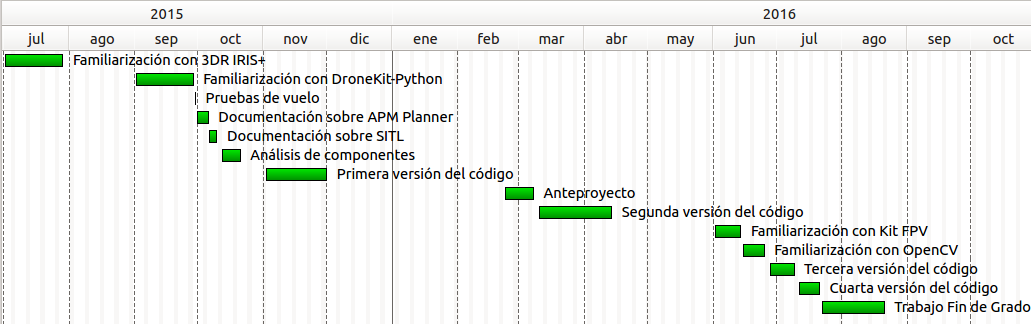
\includegraphics[width=1\textwidth]{/gantt.png}
\caption[Diagrama de distribución de tiempo por tareas en el \acs{TFG}]{Diagrama de distribución de tiempo por tareas en el \acs{TFG}}
\label{fig:gantt}
\end{center}
\end{figure}

\subsection{Fase 0: Julio 2015 - Octubre 2015}
\label{sec:primeraetapa}

En esta primera etapa, el autor debió \textbf{familiarizarse} con el componente fundamental de este proyecto, el dron 3DR IRIS+ y su entorno de desarrollo DroneKit-Python. Se realizaron \textbf{pruebas de simulación}, con código de ejemplo proporcionado por 3D Robotics. También, se hicieron \textbf{pruebas de vuelo} automáticas, en el Instituto de Tecnologías y Sistemas de Información, con el 3DR IRIS+ y la estación de control de tierra APM Planner.

Se profundizó en el estudio de APM Planner y \acs{SITL}, llevando a cabo documentos que sirvieran para dar los primeros pasos en estas plataformas.

Como última parte de esta primera etapa, se realizó un \textbf{análisis de los componentes que se necesitan} y que debían comprarse para llevar a cabo el desarrollo del proyecto. Entre otros se acordó la compra de una cámara GoPro HERO y un kit \acs{FPV}.

Entre los \textbf{problemas producidos} durante esta etapa se encuentra:
\begin{itemize}
\item \textbf{Sistema radiocontrol FlySky FS-TH9X defectuoso}: la palanca correspondiente al \textit{pitch} y al \textit{roll}, con la que se le indica al dron la dirección a la que debe moverse, llegó dañada en el envío. Esto provocaba que el dron ejecutara siempre vuelos hacia la izquierda.\\ La \textbf{solución propuesta} fue reenviar el sistema radiocontrol a 3D Robotics para ser reemplazado. El envío se realizó en Septiembre y no fue recibido de nuevo hasta Noviembre, lo que supuso dos meses sin poder trabajar con el 3DR IRIS+.
\item \textbf{Frecuencia errónea en la telemetría}: el 3DR IRIS+ cuenta con dos modelos disponibles: uno para el uso en Estados Unidos y otro para el uso en el resto del mundo. La diferencia, entre uno y otro, es la frecuencia a la que funciona la telemetría, ya que en Estados Unidos la banda que utiliza es 915 mHz y en el resto del mundo 433 mHz. En este caso, el dron fue adquirido por error con la banda de frecuencia de Estados Unidos, que en España está ocupada por el sistema de telefonía móvil \acs{GSM}. Esto provocaba una serie de interferencias, en el sistema de telemetría, que desembocaban en una lentitud considerable a la hora de cargar los parámetros del 3DR IRIS+ en la estación de control de tierra. Además, no era posible llevar a cabo la conexión con el dron real mediante esta telemetría.\\ La \textbf{solución} a este problema fue comprar una nueva telemetría que funcionara a 433 mHz.
\end{itemize}

\subsection{Fase 1: Noviembre 2015 - Febrero 2016}
\label{sec:segundaetapa}

Meses más tarde, en Noviembre de 2015 se comenzó a desarrollar la \textbf{primera versión del código}. En esta primera versión, se diseñó el sistema, mediante reuniones con David Vallejo, y se implementó el esqueleto de código que ha sido utilizado y mejorado a lo largo del proyecto. 

La primera versión del código contaba con el \textit{Coordinador}, el \textit{Proxy Dron} y el \textit{Dron}. En él, los «waypoints» eran ordenados por prioridad, divididos en listas, que dependían del número de drones que hubiera disponibles, y asignados al vehículo que le correspondiera. Es decir, no se realizaba ningún tipo de coordinación, simplemente todos los puntos de interés eran repartidos, respetando la prioridad, entre él número de vehículos existentes.

Durante el mes de Diciembre y el mes de Enero, se procedió a \textbf{pausar el proyecto} debido a los exámenes finales del primer cuatrimestre.

Entre los \textbf{problemas producidos} durante esta etapa se encuentra:
\begin{itemize}
\item \textbf{Hilos accediendo a recursos compartidos}: al hacer uso de hilos y ejecutar misiones con más de un dron, los vehículos se creaban en el mismo puerto UDP. Este inconveniente ocasionaba que todos los vehículos volaran hacia los mismos puntos de interés, haciendo inservible el empleo de más de un dron en el sistema. \\ La \textbf{solución} a este problema fue utilizar \textit{locks}, como método de sincronización, en el momento en el que se produce la conexión con el dron.
\end{itemize}

\subsection{Fase 2: Marzo 2016 - Mayo 2016}
\label{sec:terceraetapa}

En la segunda versión, se modificó la manera en que las misiones son asignadas, puesto que se introdujo el concepto de \textbf{coordinación entre drones}. Se decidió que los puntos de interés se adjudicaran a vehículos que son detectados en un estado ocioso o desocupado. De esta manera, se consiguió mejorar la productividad y el rendimiento del sistema, debido a que anteriormente un vehículo que terminaba de recorrer los «waypoints» que se le habían asignado, no colaboraba con el resto de drones en la misión. 

Además se \textbf{cambió el orden en el que se ejecutaban las operaciones de asignación de puntos de interés y de conexión} con el vehículo. Antes, los puntos de interés eran asignados a vehículos aun no conectados, lo que ocasionaba que si la conexión a un vehículo, al que se le había designado un punto de interés de alta prioridad, tardaba en realizarse, este punto de interés podría ser pasado por alto por otro vehículo cuya conexión haya sido más rápida. De forma que, se estaría incumpliendo el modelo de prioridades del sistema.

Durante el mes de Mayo se volvió a \textbf{detener el desarrollo del proyecto} a causa de los exámenes finales del segundo cuatrimestre.

Entre los \textbf{problemas producidos} durante esta etapa se encuentra:
\begin{itemize}
\item \textbf{Rotura de las patas del dron}: al efectuar el aterrizaje, tras uno de los vuelos de prueba, se parte una de las patas del dron. Esto imposibilita el uso del dron hasta tener piezas de repuesto, dado que el vehículo no dispone de una plataforma segura para el aterrizaje. \\ La \textbf{solución} a este problema fue comprar un pack de patas de repuesto para el 3DR IRIS+, pero en vista de que los pedidos de 3D Robotics tardan en llegar más de un mes, se decidió hacer uso de la impresora 3D, que existe en la Escuela Superior de Informática, para fabricar cuatro patas nuevas que permitieran volar el dron mientras los repuestos eran enviados. 
\end{itemize}

\subsection{Fase 3: Junio 2016 - Septiembre 2016}
\label{sec:cuartaetapa}

Considerando que la coordinación de \acs{UAV}s en situaciones de emergencia ha sido resuelta, con las versiones desarrolladas previamente, en esta etapa se procedió a incorporar los procedimientos para poder \textbf{capturar imágenes} que posteriormente sean \textbf{analizadas}.

Lo primero fue \textbf{familiarizarse con el kit \acs{FPV} y la biblioteca OpenCV}. Ejemplos de código, proporcionados al instalar OpenCV, fueron ejecutados y se grabaron vídeos de prueba hasta comprender que funciones eran necesarias para añadir esta funcionalidad al código del proyecto.

Se realizó una tercera versión, en la que entra en juego el \textit{Sistema FPV}, en la que se grababan las imágenes que procedían de la cámara equipada en el vehículo. Adicionalmente, se estipuló parametrizar el periodo de tiempo, en segundos, cada el que se toma una captura de pantalla de la grabación.

Por último, para realizar la cuarta y última versión del sistema fue necesario entender el funcionamiento de Google Cloud Vision \acs{API}. En la última versión del sistema, se integró el módulo de análisis de imágenes, en el que las capturas de pantalla son examinadas y se muestran por pantalla los resultados obtenidos.

Se decide entregar el \acs{TFG} en Septiembre, por lo que, el mes de Julio y Agosto fue dedicado a documentar el proyecto. Con la entrega del \acs{TFG} el proyecto se considera cerrado en Septiembre de 2016.

Entre los \textbf{problemas producidos} durante esta etapa se encuentra:
\begin{itemize}
\item \textbf{Placa de Tarot T-2D Gimbal estropeada}: mientras se llevaban a cabo pruebas de vuelo, en las que se recogían imágenes, la placa de la gimbal resultó dañada. Se trató de un problema grave, puesto que, no es posible conseguir una grabación de vídeo estable sin ella. \\ La \textbf{solución} a este problema fue comprar una nueva placa, junto con unos nuevos motores estabilizadores.
\item \textbf{Baterías para el sistema \acs{FPV} deterioradas}: para que el sistema \acs{FPV} funcione, es necesario contar con dos baterias de 1300 mAh, una para el transmisor y otra para el receptor. Dos de las tres baterías de las que se disponía, sufrieron desperfectos y dejaron de cargar. Por lo tanto, el sistema \acs{FPV} quedó inoperativo. \\ La \textbf{solución} a este problema fue comprar nuevas baterías de 1300 mAh.
\end{itemize}

\section{Casos de estudio}

Se plantean dos casos de estudio para probar el funcionamiento del sistema. 

El primero de ellos servirá para \textbf{poner a prueba el método de coordinación entre \acs{UAV}s}, para ello, se propone una situación de emergencia en la que varios drones deben cubrir, de forma conjunta, el escenario que ha sido afectado por un ataque terrorista. Al disponer de un solo vehículo aéreo, el caso se lleva a cabo mediante la ejecución de \acs{SITL}.

El segundo caso de estudio se realizará para comprobar la \textbf{operatividad completa del sistema}. Esto se debe a que, este caso de estudio se efectuará con el único dron disponible, el 3DR IRIS+. Se diseñará una misión en un entorno en la que el \acs{UAV} pueda capturar y analizar imágenes de relevancia, verificando así que el sistema es capaz de cumplir con los objetivos fijados.

Como se observa, el planteamiento propuesto consiste en \textbf{primero simular} la funcionalidad del sistema y \textbf{después ejecutar una prueba real} con el vehículo aéreo. Este enfoque, de simular antes para posteriormente realizar una prueba real, se ha seguido a lo largo de todo el desarrollo del proyecto. Gracias a esto se consigue:

\begin{itemize}
\item \textbf{Experimentar} con código implementado \textbf{sin poner en peligro la infraestructura} hardware del proyecto.
\item \textbf{Probar el código} del sistema sin hacer uso del 3DR IRIS+, lo que permite desarrollar y comprobar el funcionamiento del código \textbf{en cualquier lugar}, además de evitar posibles daños en el vehículo.
\item \textbf{Coordinar} misiones, con tantos vehículos como se desee, sin necesidad de poseer una flota de drones.
\end{itemize}

En conclusión, la mayor ventaja, de tener la posibilidad de ejecutar el sistema mediante simulaciones de \acs{UAV}s, es tener la seguridad y la certeza, a la hora de realizar pruebas con el vehículo real, de que el código se ha desarrollado correctamente y su ejecución no debería causar problemas.

Por el contrario, \textbf{la simulación no permite la captura y el análisis de imágenes}, por lo que, para probar esta funcionalidad no queda más remedio que usar el 3DR IRIS+.

\subsection{Caso de estudio 1: coordinación de \acs{UAV}s en estado de emergencia}

Para probar y \textbf{demostrar la funcionalidad del sistema}, se ha diseñado una misión en la que varios \acs{UAV}s puedan coordinarse y, de este modo, ofrecer una solución al problema de monitorizar diferentes puntos de un territorio.

Como solo se dispone de un dispositivo de vuelo real, se ha hecho uso de la \textbf{simulación de tres vehículos aéreos}, a través de \acs{SITL}, que llevarán a cabo labores de coordinación para inspeccionar de una forma más rápida el lugar.

Recordar que, al tratarse de vehículos simulados, el \textbf{\textit{Módulo de Análisis de Imágenes} no estará activo}. 

%Aún así, en el Anexo se muestran ejemplos de imágenes analizadas en diferentes entornos.

\subsubsection{Planteamiento}

El problema que se plantea es el siguiente: la \textbf{monitorización de distintos puntos} de interés dentro de una \textbf{instalación deportiva que ha sufrido un ataque terrorista}. La localización elegida, por cercanía y por familiaridad con el entorno, es el Polideportivo Juan Carlos I (ver Figura~\ref{fig:instalacion}). Sus instalaciones cuentan con:
\begin{itemize}
\item 3 campos de fútbol, con un aforo total de \textbf{4.500 personas}.
\item 3 pistas polideportivas descubiertas.
\item 1 Pabellón cubierto, con capacidad para \textbf{500 personas}.
\item 7 pistas de pádel.
\item 2 pistas de tenis.
\item 2 pistas de frontón.
\item 1 piscina cubierta, con aforo para \textbf{250 personas}.
\item 1 piscina descubierta. \\
\end{itemize}

\begin{figure}[!h]
\begin{center}
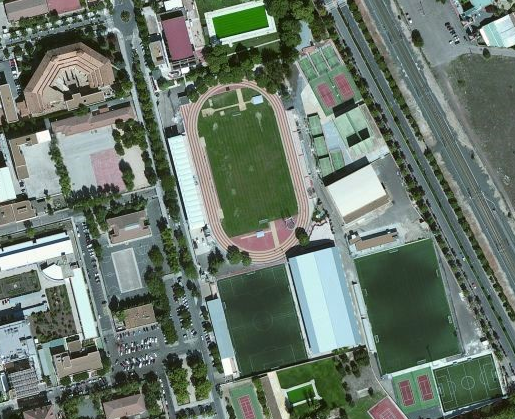
\includegraphics[width=0.8\textwidth]{/instalacion.png}
\caption[Polideportivo Juan Carlos I]{Polideportivo Juan Carlos I}
\label{fig:instalacion}
\end{center}
\end{figure}

En definitiva, se trata de una ubicación en la que, en un momento dado, puede existir una \textbf{gran confluencia de gente}. Por lo que, tras un posible ataque terrorista es adecuada la utilización de drones, para recolectar información del entorno que sea de utilidad para los equipos de emergencia.

\subsubsection{Diseño de la solución}

Para cubrir el mayor terreno posible en el menor tiempo, se siguen estas pautas:

\begin{itemize}
\item Se fijan tres puntos, en los extremos de la instalación deportiva, con una prioridad de 1. Con esto lo que se pretende, es que los drones acudan \textbf{primero a las ubicaciones más lejanas} para que después vayan cerrando, de forma coordinada, el radio de actuación. En caso contrario, un dron podría tener que recorrer una gran distancia, haciendo el sistema menos eficiente.
\item Se fijan tres puntos, cercanos a las ubicaciones anteriores, con una prioridad de 2. De este modo, se consigue que el \textbf{radio de actuación se estreche}, posibilitando que, posteriormente, al resto de puntos pueda volar cualquier vehículo sin que esté demasiado lejos.
\item El resto de puntos se fijan con una prioridad de 3. Los vehículos vuelan a una distancia cercana entre ellos, por lo tanto, el vuelo a \textbf{cualquier ubicación no supondrá una pérdida de tiempo elevada}.
\end{itemize}

\begin{figure}[!h]
\begin{center}
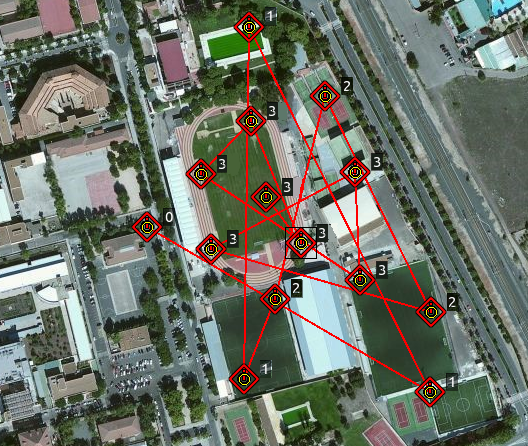
\includegraphics[width=0.73\textwidth]{/mision.png}
\caption[Diseño de la misión en el Polideportivo Juan Carlos I]{Diseño de la misión en el Polideportivo Juan Carlos I}
\label{fig:mision}
\end{center}
\end{figure}

\subsubsection{Ejecución de la solución}

Para comenzar el vuelo de los vehículos, que van a ejecutar la misión diseñada, se debe \textbf{llamar por línea de comandos a \textit{Coordinator.py}} con el parámetro de vehículos a 3 (ver Listado~\ref{code:iniciosimulacion}).

\begin{listing}[
 float=h!,
 language = bash,
 caption = {Inicio del sistema para simulación de tres vehículos},
 label  = code:iniciosimulacion]
$ python coordinator.py --vehicles 3
\end{listing}

Al realizar está llamada, el sistema desplegará tres ventanas (ver Figura~\ref{fig:despliegue}), que se corresponden con los vehículos simulados, mientras que en la terminal de Ubuntu se ofrece información del sistema y de los drones como, por ejemplo: 
\begin{itemize}
\item Creación de objetos del sistema.
\item Realización del despegue.
\item LLegada a puntos de interés.
\item Realización del aterrizaje.
\item Puntos de interés visitados por cada \acs{UAV}.
\end{itemize}

\begin{figure}[!h]
\begin{center}
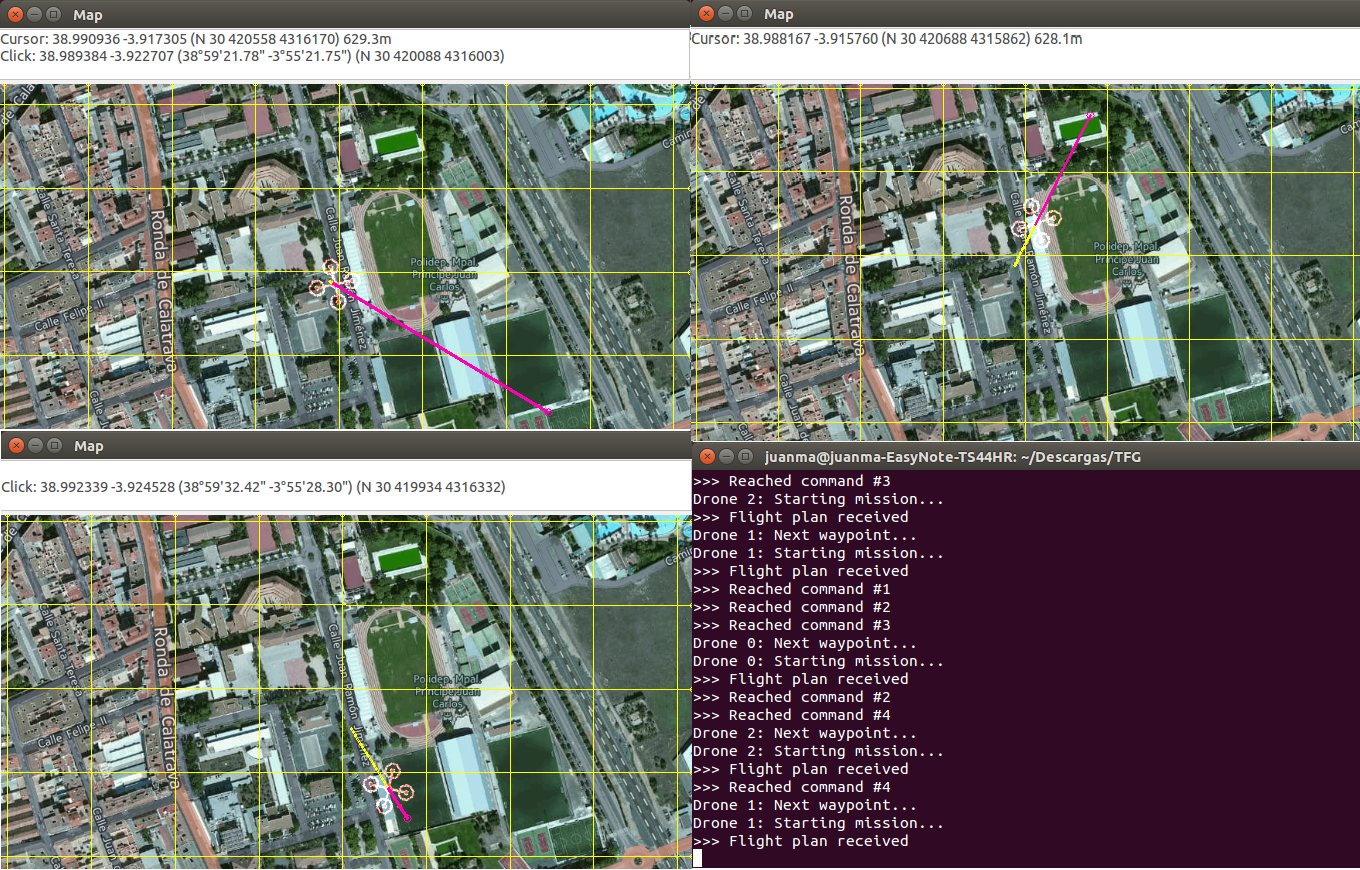
\includegraphics[width=0.8\textwidth]{/despliegue.png}
\caption[Despliegue del sistema con tres drones]{Despliegue del sistema con tres drones}
\label{fig:despliegue}
\end{center}
\end{figure}

El sistema seguirá la solución que se ha diseñado, de tal forma que el \textbf{dron 1 volará a cuatro puntos de interés} (ver Figura~\ref{fig:dron1}).

\begin{figure}[!h]
\begin{center}
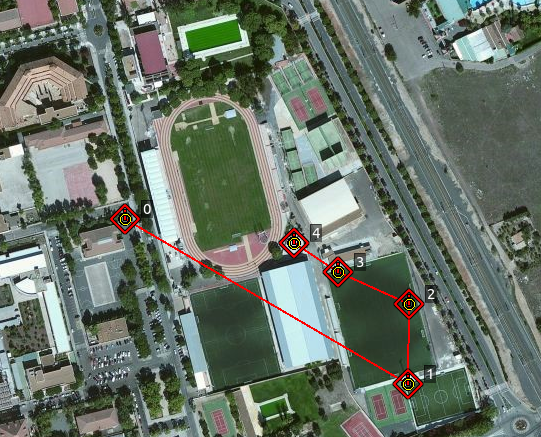
\includegraphics[width=0.8\textwidth]{/dron1.png}
\caption[Misión realizada por el dron 1]{Misión realizada por el dron 1}
\label{fig:dron1}
\end{center}
\end{figure}

El \textbf{dron 2 también visitará cuatro puntos de interés} antes de volver a la zona de despegue (ver Figura~\ref{fig:dron2}).

\begin{figure}[!h]
\begin{center}
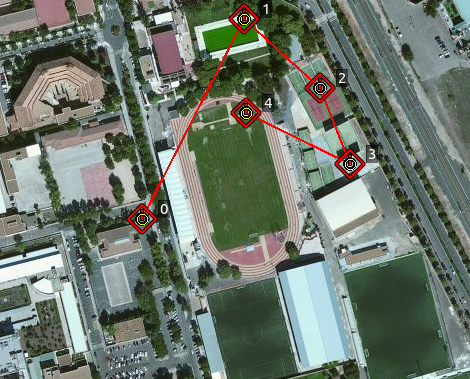
\includegraphics[width=.8\textwidth]{/dron2.png}
\caption[Misión realizada por el dron 2]{Misión realizada por el dron 2}
\label{fig:dron2}
\end{center}
\end{figure}

Por último, el \textbf{dron 3 acudirá a cinco puntos de interés} (ver Figura~\ref{fig:dron3}).

\begin{figure}[!h]
\begin{center}
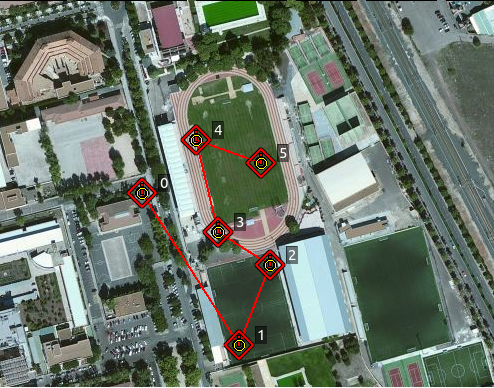
\includegraphics[width=0.8\textwidth]{/dron3.png}
\caption[Misión realizada por el dron 3]{Misión realizada por el dron 3}
\label{fig:dron3}
\end{center}
\end{figure}

%Se pueden consultar las imágenes de la realización de la misión punto por punto en el Anexo .

\subsubsection{Conclusión del caso de estudio}

Después de la ejecución de la solución haciendo uso del sistema desarrollado, se obtienen una serie de conclusiones:

\begin{itemize}
\item Se confirma que la coordinación de varios \acs{UAV}s es una funcionalidad fundamental en situaciones de catástrofe. Utilizando tres drones, el tiempo para recorrer todos los puntos de la misión ha sido de 4 minutos y 30 segundos. Esto quiere decir, que en menos de 5 minutos los equipos de emergencia podrían haber dispuesto de información vital acerca del escenario. En cambio, haciendo uso de un solo vehículo, el tiempo para recorrer los puntos de interés por prioridad asciende hasta algo más de 13 minutos. Así pues, gracias al despliegue de varios drones se consigue \textbf{reducir el tiempo de actuación en un tercio}.
\item Es \textbf{esencial un buen diseño a la hora de crear la misión}. Una misión en la que un dron acuda a un punto de prioridad, que se encuentra lejos de su ubicación, existiendo uno más cercano, de la misma prioridad, convierte el sistema en menos eficiente. Por ello, es primordial fijar los puntos de interés en un buen orden de ejecución. Por ejemplo, en el supuesto del caso de estudio, cerrando poco a poco el radio de actuación.
\end{itemize}

\clearpage

\subsection{Caso de estudio 2: ejecutando el sistema sobre el 3DR IRIS+}

Para verificar y \textbf{confirmar que el sistema cumple con los objetivos propuestos}, se creará una misión con varios «waypoints» en la que, usando el vehículo aéreo 3DR IRIS+, el sistema haga volar el dron hasta cada uno de ellos y consiga capturar y analizar las imágenes tomadas desde el \acs{UAV}. 

En este caso de estudio se demostrará el resultado real, al ejecutar una misión con el 3DR IRIS+, del sistema desarrollado en este \acs{TFG}.

\subsubsection{Planteamiento}

Al hacer uso del 3DR IRIS+, cuyo peso no excede los 25 kg, se deben seguir una serie de \textbf{normas establecidas en la Normativa Española de Seguridad Aérea} (ver Anexo \ref{chap:normativa}):

\begin{itemize}
\item Operar en zonas \textbf{fuera de aglomeraciones}, de edificios y personas, en ciudades, pueblos o lugares habitados.
\item Operar a una \textbf{altura} sobre el terreno \textbf{no mayor de 120 metros}.
\item Volar \textbf{dentro del alcance visual} del piloto, a una distancia de éste no mayor de 500 metros
\end{itemize}

Siguiendo esta reglas, la misión se proyecta sobre una parcela desocupada, de personas e infraestructuras, a las afueras de Ciudad Real (ver Figura~\ref{fig:instalacion2}).

\begin{figure}[!h]
\begin{center}
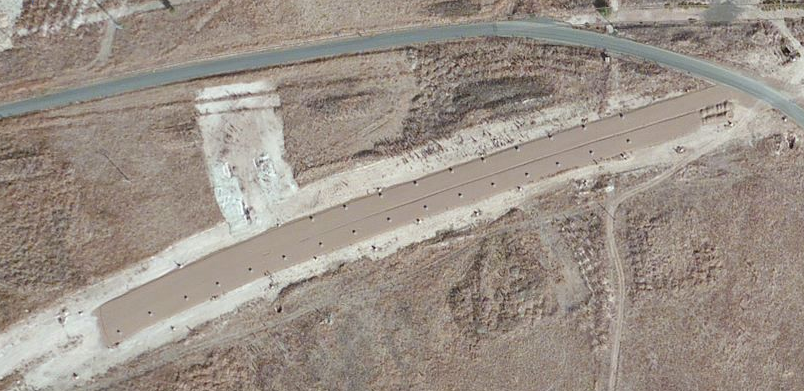
\includegraphics[width=0.8\textwidth]{/casoestudio2.png}
\caption[Extensión donde ejecutar el caso de estudio]{Extensión donde ejecutar el caso de estudio}
\label{fig:instalacion2}
\end{center}
\end{figure}

La ubicación elegida cumple con la Normativa Española de Seguridad Aérea, pero debido a este reglamento tan estricto, es \textbf{difícil} poder \textbf{capturar imágenes de cierta relevancia} que sean analizadas por \textit{Google Cloud Vision \acs{API}}.

\subsubsection{Diseño de la solución}

Puesto que en este caso de estudio no es necesario coordinar varios vehículos, siendo lo realmente importante que el \textbf{3DR IRIS+ vuele a los «waypoints» mientras recoge y analiza imágenes}, simplemente se fijarán tres puntos de interés en la zona antes mencionada, cada uno de una prioridad distinta, para que el 3DR IRIS+ acuda a cada uno de ellos y capture imágenes del entorno.

\begin{figure}[!h]
\begin{center}
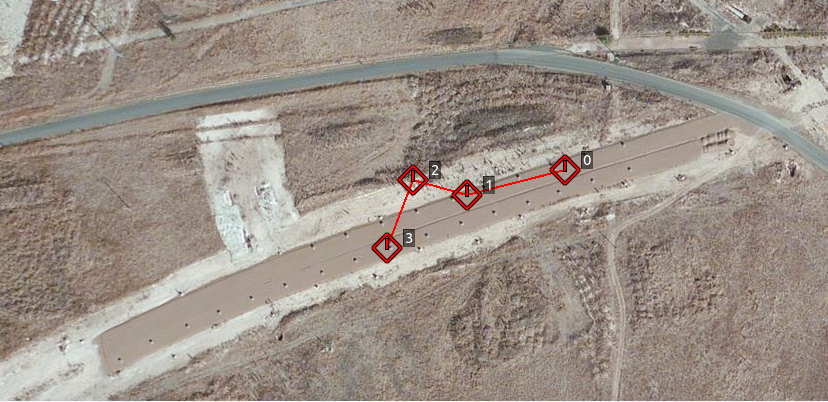
\includegraphics[width=0.8\textwidth]{/mision2.png}
\caption[Diseño de la misión del caso de estudio 2]{Diseño de la misión del caso de estudio 2}
\label{fig:mision2}
\end{center}
\end{figure}

\subsubsection{Ejecución de la solución}

Antes de iniciar la llamada al sistema, se deben \textbf{verificar ciertos aspectos} como: haber conectado la telemetría, para así, ser capaces de comunicarse con el dron o  asegurarse de que el mando radiocontrol esté operativo, debido a que, en caso de que el \acs{UAV} tenga algún fallo se pueda ordenar inmediatamente la vuelta al punto de despegue, evitando así daños en el aparato.

Para iniciar el sistema, que debe llevar a cabo la misión diseñada, se debe \textbf{llamar por línea de comandos a \textit{Coordinator.py}}, en este caso con el parámetro de vehículos a 1, el parámetro de espera en el punto de interés a 20 y el parámetro de segundos entre fotos a 5 (ver Listado~\ref{code:iniciocasoestudio2}). De este modo, se conseguirá que el sistema despliegue un solo vehículo que realizará y analizará una foto cada 5 segundos, esperando en los «waypoints» especificados un tiempo de 20 segundos.

\begin{listing}[
 float=h!,
 language = bash,
 caption = {Inicio del sistema para caso de estudio 2},
 label  = code:iniciocasoestudio2]
$ python coordinator.py --vehicles 1 --secondWait 20 --secondsPerPhoto 5
\end{listing}

\clearpage

Cuando se realiza está llamada, el sistema desplegará tres ventanas (ver Figura~\ref{fig:despliegue2}): la primera se corresponde con el 3DR IRIS+, la segunda con el sistema \acs{FPV} que muestra y analiza las imágenes y la tercera es la terminal de Ubuntu que ofrece información del sistema y del \acs{UAV}.

\begin{figure}[!h]
\begin{center}
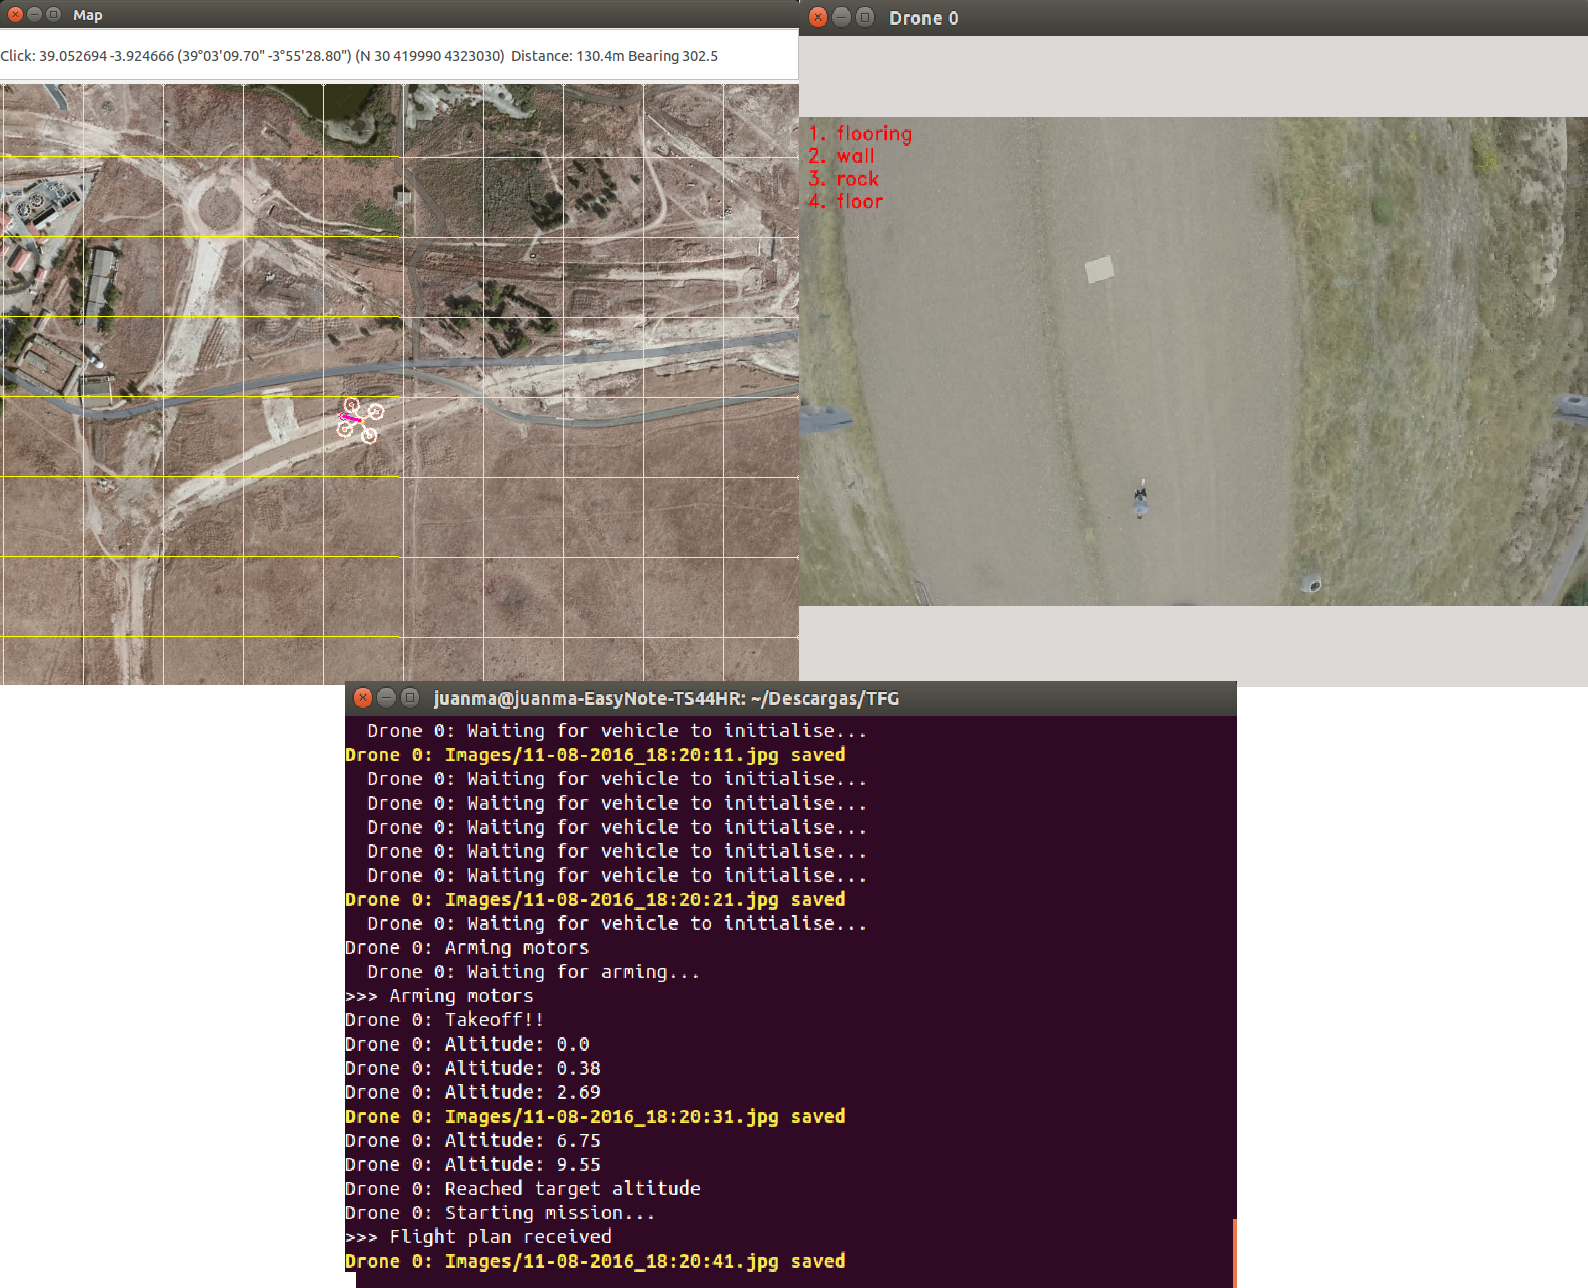
\includegraphics[width=1\textwidth]{/despliegue2.png}
\caption[Despliegue del sistema con tres drones]{Despliegue del sistema con tres drones}
\label{fig:despliegue2}
\end{center}
\end{figure}

El sistema desarrollado hará despegar el 3DR IRIS+ para que vuele hasta los puntos de interés (ver Figura~\ref{fig:1}), que se han determinado en el diseño de la misión, de tal forma que a lo largo del vuelo grabará y analizará las imágenes que está capturando (ver Figura~\ref{fig:imagen1}). \\

\begin{figure}[!h]
\begin{center}
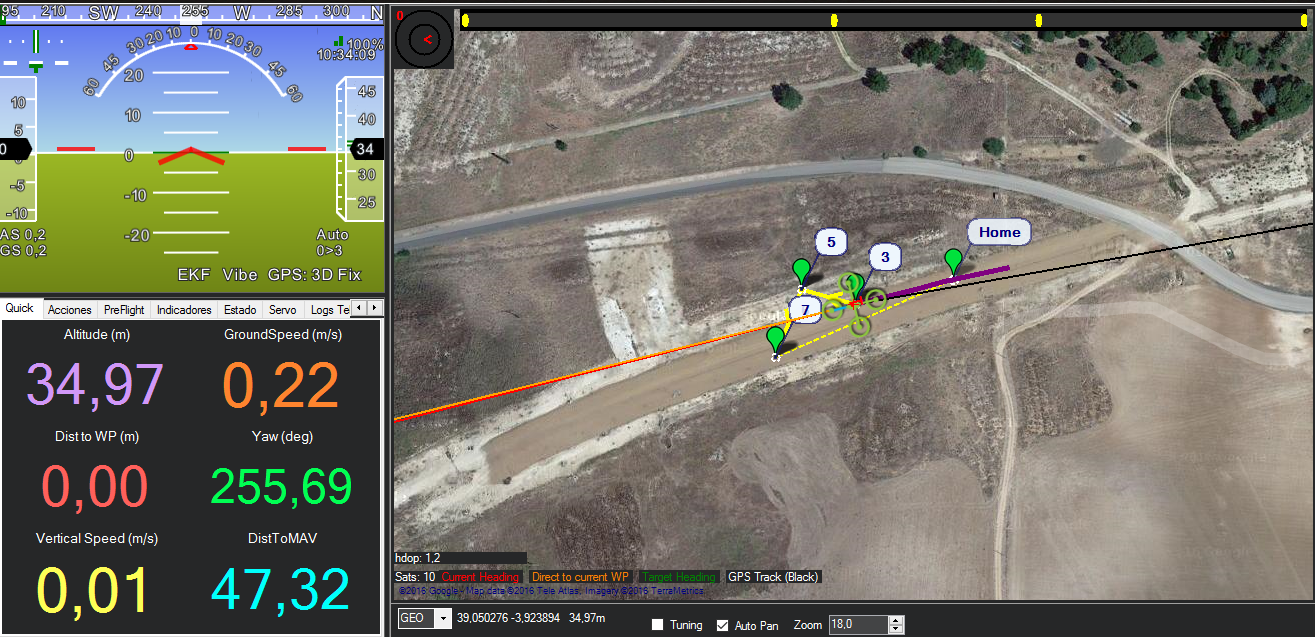
\includegraphics[width=.8\textwidth]{/1.png}
\caption[3DR IRIS+ volando a «waypoint»]{3DR IRIS+ volando a «waypoint» \footnotemark} 
\label{fig:1}
\end{center}
\end{figure}

\footnotetext{Para una mejor comprensión del vuelo del vehículo, se muestran capturas de pantalla de Mission Planner}

\begin{figure}[!h]
\begin{center}
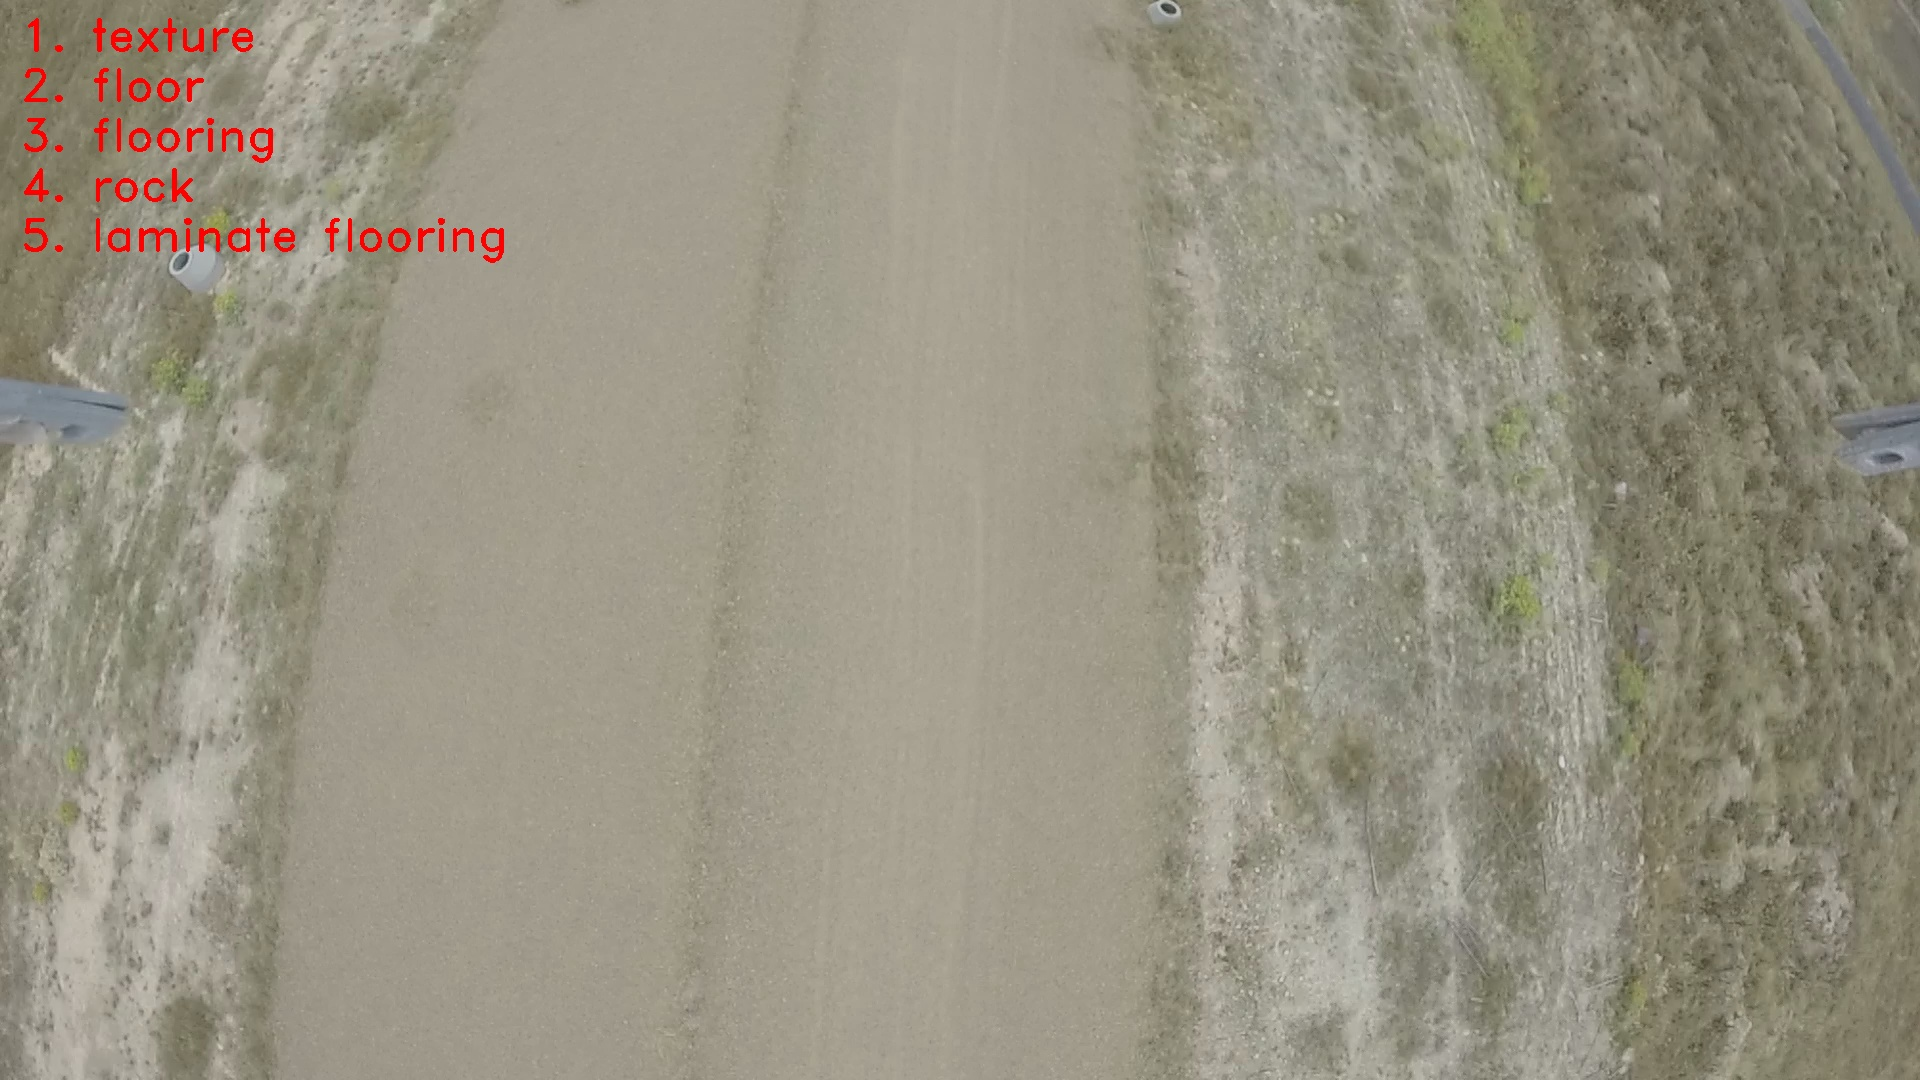
\includegraphics[width=.8\textwidth]{/resultado1.jpg}
\caption[Imagen capturada y analizada por el sistema]{Imagen capturada y analizada por el sistema}
\label{fig:imagen1}
\end{center}
\end{figure}

El resto de imágenes de la ejecución del caso de estudio se encuentran en el Anexo \ref{chap:imagenes}. Debido a las limitaciones que impone la Normativa Española de Seguridad Aérea, como tener que operar en zonas deshabitadas, es complejo poder obtener imágenes de cierta relevancia. Es por ello que, en el Anexo \ref{chap:imagenes} también se muestran imágenes extraídas de internet, de manera que, el \textit{Módulo de Análisis de Imágenes} pueda ser probado con imágenes que contienen mayor información.

%Se pueden consultar las imágenes de la realización de la misión punto por punto en el Anexo .

\subsubsection{Conclusión del caso de estudio}

Tras haber ejecutado en el sistema el segundo caso de estudio, las conclusiones obtenidas son:

\begin{itemize}
\item La \textbf{captura de imágenes aéreas debe ser un pilar fundamental en situaciones de catástrofe}. La posibilidad de contar con un \acs{UAV} que pueda inspeccionar de manera rápida, y coordinada, una porción del terreno afectado por un desastre, proporciona grandes ventajas a los equipos de emergencia. Gracias a la información que proporcionan estas imágenes, los equipos de emergencia pueden localizar a supervivientes y elaborar un plan de rescate mucho más apropiado y en un tiempo menor.
\item El \textbf{análisis de imágenes puede llegar a ser una funcionalidad vital} del sistema. Actualmente, el \textit{Módulo de Análisis de Imágenes} está enfocado a proporcionar información adicional, de tal forma que, sirva como ayuda al personal de rescate. Esto se debe a que, \textit{Google Cloud Vision \acs{API}} fue lanzado en versión beta en febrero de 2016, de modo que, los resultados que proyecta tienen un margen de mejora grande. Quizás en un futuro muy lejano, la detección de supervivientes se pueda realizar de manera automática mediante el uso de esta \acs{API}.
\end{itemize}


\section{Costes}

Es complicado dar un valor exacto al coste del proyecto, a causa de que los ciclos de trabajo no han sido constantes durante todo el desarrollo del sistema. Varias circunstancias han contribuido a que se detenga o se aminore, en varias ocasiones, la actividad del proyecto. Algunos de estas circunstancias son:

\begin{itemize}
\item Fases en las que se debía esperar la llegada de algún repuesto para poder hacer uso del sistema.
\item Periodos de exámenes.
\item Fechas en las que se debían entregar prácticas y trabajos de distintas asignaturas.
\item Compaginación con contrato deportivo.
\end{itemize}  

Por esta razón, se hará una estimación en la que se tase el coste del proyecto atendiendo a las siguientes pautas:

\begin{itemize}
\item Sueldo de un programador en Python: el salario se encuentra establecido en \textbf{20 euros por hora}.
\item El proyecto ha supuesto 13 meses de desarrollo, de los cuales se atribuyen \textbf{6 meses como productivos} al descontar los periodos de exámenes, las vacaciones y la espera hasta la llegada de repuestos.
\item Se establece un horario laboral de \textbf{37,5 horas semanales}.
\item El coste de los dispositivos hardware (ver Cuadro~\ref{tab:costes}) necesarios para elaborar el \acs{TFG}: la suma de la compra de todos los componentes asciende a \textbf{1.845,21 euros}.
\end{itemize}

Así pues, \textbf{el coste del proyecto se estima en 19.845,21 euros}.

\begin{table}[!h]
 \centering
 {\small
 \begin{tabular}{p{.59\textwidth}p{.07\textwidth}p{.12\textwidth}p{.12\textwidth}}
  \tabheadformat
  \tabhead{Componente} &
  \tabhead{Cantidad} & 
  \tabhead{Precio/Unidad} & 
  \tabhead{Precio Total} \\
\hline
\textit{3DR IRIS+}  & 1 & 660,00 \euro & 660,00 \euro \\
                 
\hline
\textit{Maleta para 3DR IRIS+}  & 1 & 250,57 \euro & 250,57 \euro \\

\hline
\textit{GoPro HERO 3+ Silver Edition}  & 1 & 295,00 \euro & 295,00 \euro \\

\hline
\textit{Tarot Gimbal TL2D01}  & 1 & 187,92 \euro & 187,92 \euro \\

\hline
\textit{3DR FPV Video/OSD System Kit}  & 1 & 169,13 \euro & 169,13 \euro \\

\hline
\textit{LogiLink USB 2.0}  & 1 & 16,12 \euro & 16,12 \euro \\

\hline
\textit{Tarot Gimbal GoPro Video Cable}  & 1 & 10,00 \euro & 10,00 \euro \\

\hline
\textit{Telemetría Flug51 FL1515 433 MHz}  & 1 & 37,70 \euro & 37,70 \euro \\
       
\hline
\textit{Patas altas para IRIS+}  & 1 & 22,36 \euro & 22,36 \euro \\

\hline
\textit{Batería LiPo 1300 mAh 3S}  & 2 & 10,95 \euro & 21,90 \euro \\

\hline
\textit{Cargador profesional iMAX B6 Mini}  & 1 & 39,40 \euro & 39,40 \euro \\

\hline
\textit{Adaptador de corriente para iMAX B6 Mini}  & 1 & 21,10 \euro & 21,10 \euro \\

\hline
\textit{Motor de repuesto TL68A06 para Tarot Gimbal}  & 1 & 10,94 \euro & 10,94 \euro \\

\hline
\textit{Motor de repuesto TL68A09 para Tarot Gimbal}  & 1 & 9,59 \euro & 9,59 \euro \\

\hline
\textit{Placa de repuesto ZYX22 para Tarot Gimbal}  & 1 & 38,48 \euro & 38,48 \euro \\

\hline
\textit{Motores y hélices de repuesto  MN2213+T9545 para IRIS+}  & 1 & 55,00 \euro & 55,00 \euro \\
\hline


\hline
 &  & \textbf{TOTAL} & \textbf{1.845,21 \euro} \\

\hline
\end{tabular}

 }
 \caption[Desglose de costes de los dispositivos hardware]
 {Desglose de costes de los dispositivos hardware}
 \label{tab:costes}
\end{table}


% Local Variables:
% coding: utf-8
% mode: latex
% mode: flyspell
% ispell-local-dictionary: "castellano8"
% End:
